%----------------------------------------------------------------------------------------
%	CHAPTER - HOW TO USE LATEX
%----------------------------------------------------------------------------------------

\chapter{Chapter Title Here} % Main chapter title

\label{Chapter1} % For referencing the chapter elsewhere, use \ref{Chapter1} 

%\lhead{Chapter x. \emph{Chapter Title Here}} % This is for the header on each page - perhaps a shortened title

%----------------------------------------------------------------------------------------

\section{Learning \LaTeX{}}

\LaTeX{} is not a WYSIWYG (What You See is What You Get) program, unlike word processors such as Microsoft Word or Apple's Pages. Instead, a document written for \LaTeX{} is actually a simple, plain text file that contains \emph{no formatting}. You tell \LaTeX{} how you want the formatting in the finished document by writing in simple commands amongst the text, for example, if I want to use \textit{italic text for emphasis}, I write the `$\backslash$\texttt{textit}\{\}' command and put the text I want in italics in between the curly braces. This means that \LaTeX{} is a ``mark-up'' language, very much like HTML.

\subsection{A (not so short) Introduction to \LaTeX{}}

If you are new to \LaTeX{}, there is a very good eBook -- freely available online as a PDF file -- called, ``The Not So Short Introduction to \LaTeX{}''. The book's title is typically shortened to just ``lshort''. You can download the latest version (as it is occasionally updated) from here:\\
\href{http://www.ctan.org/tex-archive/info/lshort/english/lshort.pdf}{\texttt{http://www.ctan.org/tex-archive/info/lshort/english/lshort.pdf}}

It is also available in several other languages. Find yours from the list on this page:\\
\href{http://www.ctan.org/tex-archive/info/lshort/}{\texttt{http://www.ctan.org/tex-archive/info/lshort/}}

It is recommended to take a little time out to learn how to use \LaTeX{} by creating several, small `test' documents. Making the effort now means you're not stuck learning the system when what you \emph{really} need to be doing is writing your thesis.

\subsection{A Short Math Guide for \LaTeX{}}

If you are writing a technical or mathematical thesis, then you may want to read the document by the AMS (American Mathematical Society) called, ``A Short Math Guide for \LaTeX{}''. It can be found online here:\\
\href{http://www.ams.org/tex/amslatex.html}{\texttt{http://www.ams.org/tex/amslatex.html}}\\
under the ``Additional Documentation'' section towards the bottom of the page.

\subsection{Common \LaTeX{} Math Symbols}
There are a multitude of mathematical symbols available for \LaTeX{} and it would take a great effort to learn the commands for them all. The most common ones you are likely to use are shown on this page:\\
\href{http://www.sunilpatel.co.uk/latexsymbols.html}{\texttt{http://www.sunilpatel.co.uk/latexsymbols.html}}

You can use this page as a reference or crib sheet, the symbols are rendered as large, high quality images so you can quickly find the \LaTeX{} command for the symbol you need.

%----------------------------------------------------------------------------------------

\section{What this Template Includes}

\subsection{Folders}

\textbf{01\_Chapters} -- this is the folder where you put the thesis chapters. The number of chapters is depending on the number of chapters needed for the \textit{Body of Text}. Each chapter should go in its own separate `\texttt{.tex}' file and they usually are split as:

\begin{itemize}
    \item Chapter 1: Introduction
    \item Chapter 2: Literature review
    \item Chapter 3: Research Method
    \item Chapter 4: Body of Text (1)
    \item Chapter 5: Body of Text (2)
    \item Chapter 6: Body of Text (3)
    \item Chapter 7: Conclusion
\end{itemize}

\textbf{02\_Appendices} -- this is the folder where you put the appendices. Each appendix should go into its own separate `\texttt{.tex}' file. A template is included in the directory.

\textbf{03\_Figures} -- this folder contains all figures (e.g.~pictures, diagrams, visualisations, etc.) for the thesis. These are the final images that will go into the thesis document.

\textbf{04\_Packages} -- this folder contains missing \LaTeX{} packages (`\texttt{.sty}' file) that are needed to compile this thesis document.

\subsection{Files}

Included are also several files, most of them are plain text and you can see their contents in a text editor. Luckily, many of them are auxiliary files created by \LaTeX{} or BibLaTeX and which you don't need to bother about. Important files are:

\textbf{Author-Year-Title.pdf} -- This is your beautifully typeset thesis (in the PDF file format) created by \LaTeX{}.

\textbf{Author-Year-Title.tex} -- This is the file that you tell \LaTeX{} to compile to produce your thesis as a PDF file. It contains the framework and constructs that tell \LaTeX{} how to layout the thesis. It is heavily commented so you can read exactly what each line of code does and why it is there.

\textbf{Bibliography.bib} -- File that contains all the bibliographic information and references that you will be citing in the thesis for use with BibLaTeX. You can write it manually, but there are reference manager programs available that will create and manage it for you. Bibliographies in \LaTeX{} are a large subject and you may need to read about BibTeX/BibLaTeX before starting with this.

\textbf{Thesis.cls} -- Style file that tells \LaTeX{} how to format the thesis. It is not necessary to change this file, so please leave it as it is.

%----------------------------------------------------------------------------------------

\section{Thesis Features and Conventions}
\label{ThesisConventions}

\subsection{Printing Format}

This thesis template is designed for single sided printing as most theses are printed and bound this way. This means that the left margin is always wider than the right (for binding). Four out of five people will now judge the margins by eye and think, ``I never 
noticed that before.''.

The headers for the pages contain the page number on the right side (so it is easy to flick through to the page you want) and the chapter name on the left side.

The text is set to 11 point and a line spacing of 1.3. Generally, it is much more readable to have a smaller text size and wider gap between the lines than it is to have a larger text size and smaller gap.

\subsection{References}

The \textit{American Psychological Association~(APA)} package of BibLaTeX is used to format the bibliography. The first in-text reference appears like that~\textcite{Reference1}, while the following references appear like that~\textcite{Reference1}. The same principle is applied for the first reference in brackets~\parencite{Reference3}, while the following references appear like that~\parencite{Reference3}. However, you can also cite multiple references (in alphabetical order) at one once like that~\textcite{Reference1,Reference2} or that~\parencite{Reference1,Reference2}. Further information regarding citation in LaTeX{} can be found \href{http://en.wikibooks.org/wiki/LaTeX/Bibliography_Management}{here} or \href{http://www.ctan.org/pkg/apa6}{here}.

Scientific references should come \emph{before} the punctuation mark if there is one (such as a comma or period) together with a \verb!~! in front of the citation command. The same goes for footnotes\footnote{Such as this footnote, here down at the bottom of the page.}. You can change this but the most important thing is to keep the convention consistent throughout the thesis. Footnotes themselves should be full, descriptive sentences (beginning with a capital letter and ending with a full stop).

Did you know that Mendeley is supporting \LaTeX{}? If not have a look at this \href{http://blog.mendeley.com/tipstricks/howto-use-mendeley-to-create-citations-using-latex-and-bibtex/}{blog post} and get to know the power of these powerful tools.

\subsection{Glossary and Abbreviations}

You can reference any glossary term that you have defined at the beginning of this document, by the following commands `$\backslash$\texttt{gls}' (singular) or `$\backslash$\texttt{glspl}' (plural). An example is provided below:

In addition to that is also possible to reference any abbreviations in the same way. However, if you reference an abbreviation the first time it will show you the full name plus the abbreviation itself in the brace. From the second time you reference the same abbreviation it will only show you the abbreviation itself. An example is provided below:


Further information regarding glossary and abbreviations can be found \href{http://www.ctan.org/pkg/glossaries}{here} and \href{http://latex-community.org/know-how/latex/55-latex-general/263-glossaries-nomenclature-lists-of-symbols-and-acronyms}{here}.

\subsection{Figures}

There will hopefully be many figures in your thesis (that should be placed in the `03\_Figures' folder). The way to insert figures into your thesis is to use a code template like this:

\begin{verbatim}
\begin{figure}[htbp]
	\centering
		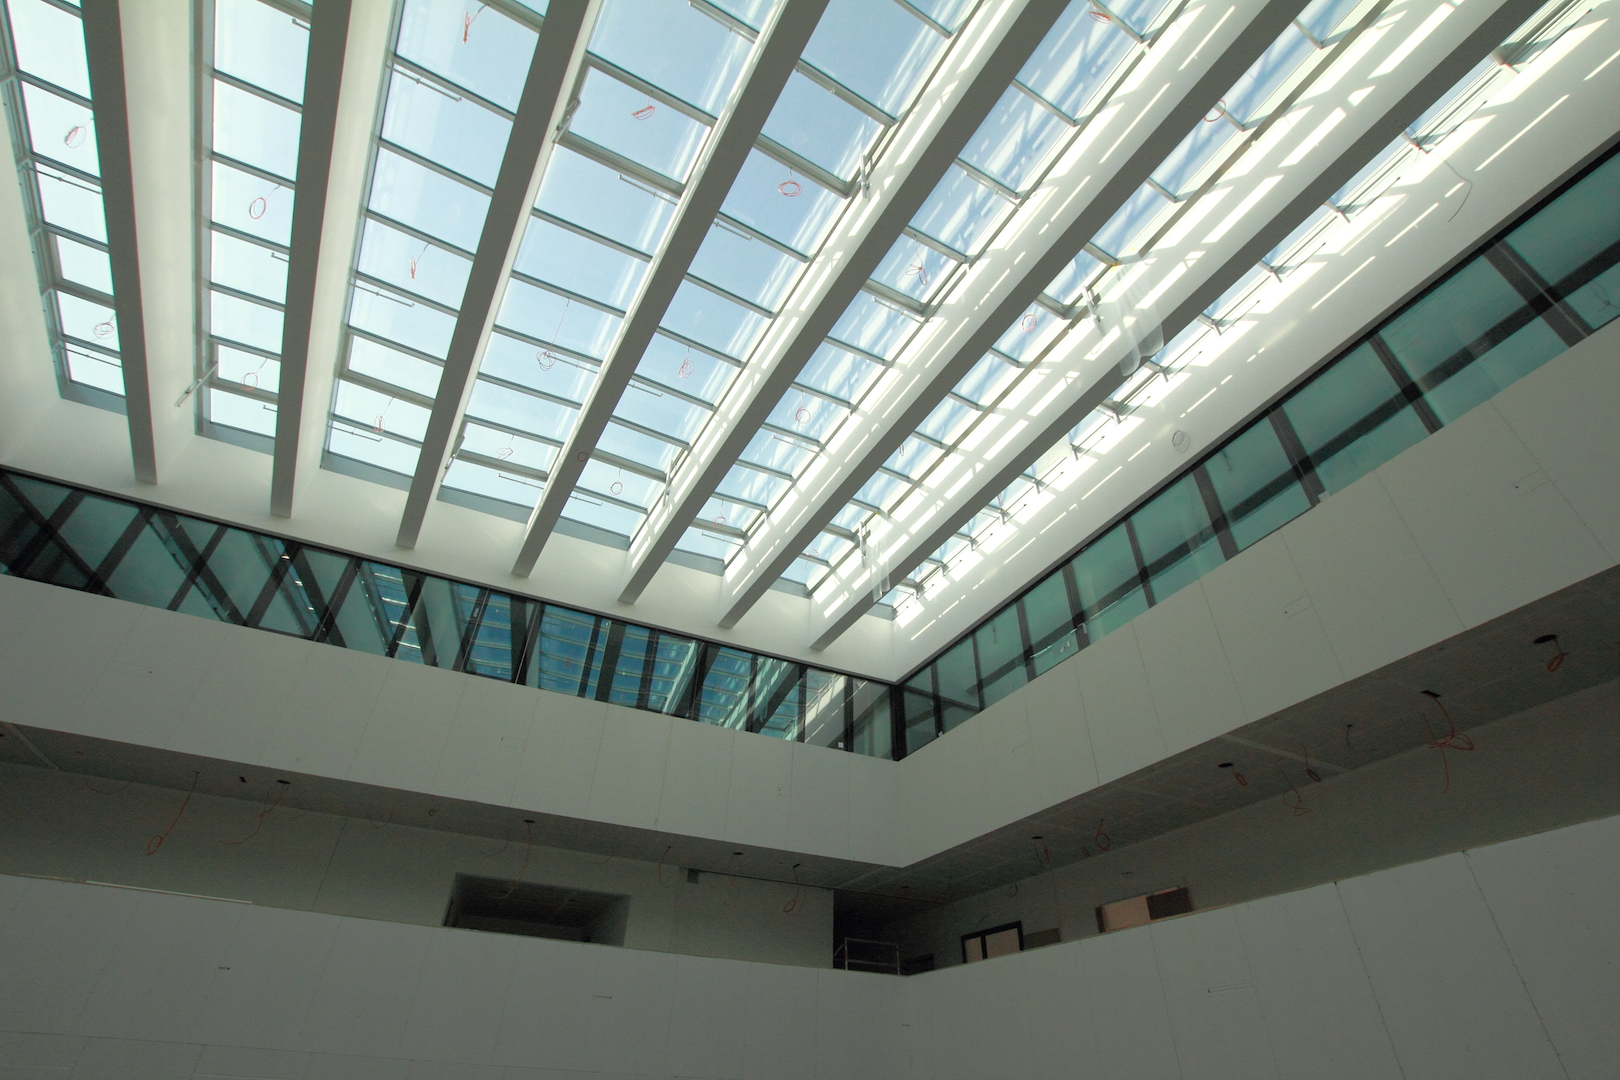
\includegraphics[width=13cm]{01_Campus/CampusOlten.jpeg}
		\rule{35em}{0.5pt}
	\caption[Campus Olten]{FHNW Campus Olten.}
	\label{fig:Campus}
\end{figure}
\end{verbatim}

Also look in the source file. Putting this code into the source file produces the picture of the electron that you can see in the figure below.

\begin{figure}[htbp]
	\centering
		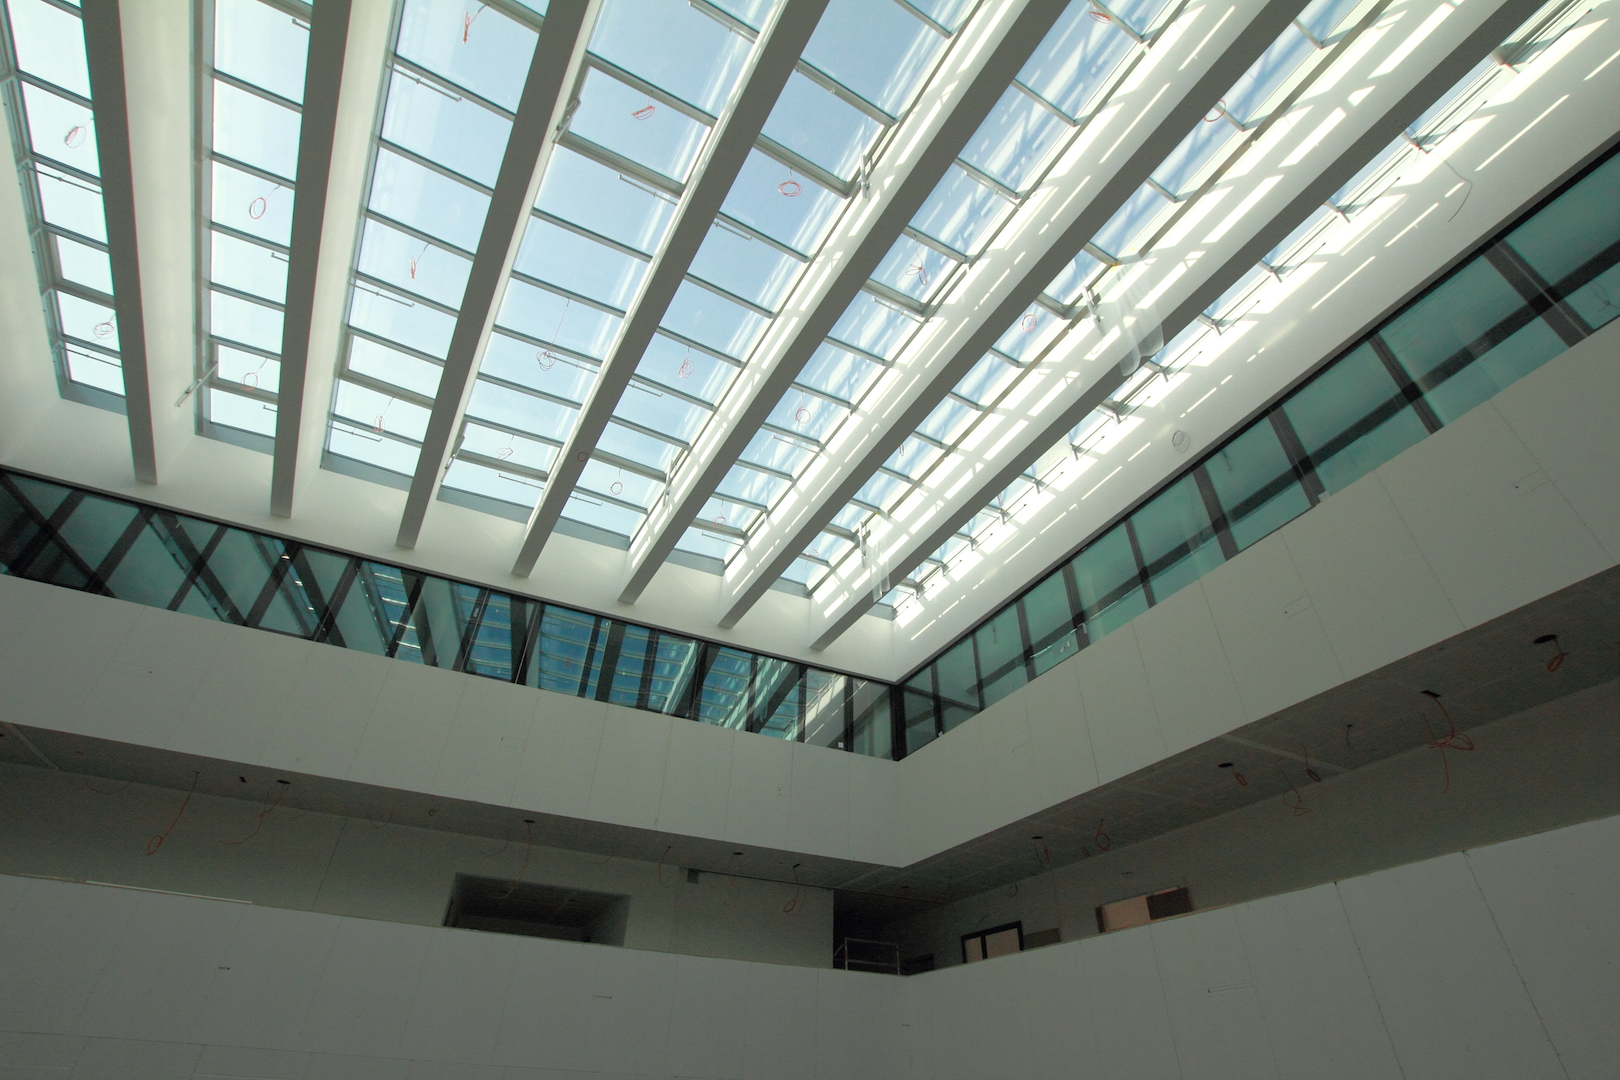
\includegraphics[width=10cm]{01_Campus/CampusOlten.jpeg}
		\rule{35em}{0.5pt}
	\caption[Campus Olten]{FHNW Campus Olten.}
	\label{fig:Campus}
\end{figure}

Sometimes figures don't always appear where you write them in the source. The placement depends on how much space there is on the page for the figure. Sometimes there is not enough room to fit a figure directly where it should go (in relation to the text) and so \LaTeX{} puts it at the top of the next page. Positioning figures is the job of \LaTeX{} and so you should only worry about making them look good!

Figures usually should have labels just in case you need to refer to them (such as in Figure \ref{fig:Campus}). The `$\backslash$\texttt{caption}' command contains two parts, the first part, inside the square brackets is the title that will appear in the `List of Figures', and so should be short. The second part in the curly brackets should contain the longer and more descriptive caption text.

The `$\backslash$\texttt{rule}' command is optional and simply puts an aesthetic horizontal line below the image. If you do this for one image, do it for all of them.

The \LaTeX{} Thesis Template is able to use figures that are either in the PDF or JPEG file format.

\subsection{Tables}

\LaTeX{} is capable to create beautiful tables from scratch, to improve them even more we implemented the \texttt{booktabs} package for you. Further information regarding this package and why it's not recommend to use horizontal lines can be found \href{http://texdoc.net/texmf-dist/doc/latex/booktabs/booktabs.pdf}{here}.

Tables are in many ways like figures as such it is also possible to define the position, to attach a caption or to add a label (see Table \ref{table:FHNWLocations}). The number of rows respectively their size and behaviour can be defined in the header of the within the `$\backslash$\texttt{tabular}' command. In this example we have defined two top-aligned paragraphs with a predefined size. Further row types and explanations can be found \href{http://en.wikibooks.org/wiki/LaTeX/Tables}{here}. 

The \texttt{booktabs} package offers furthermore the opportunity to define a horizontal line at the beginning (\verb!\toprule!), between (\verb!\midrule!) and the end (\verb!\bottomrule!) of the table. 

However, in order to start a new column you can simply add a \texttt{\$} at the end of your current column. In the same way you can also start a new row by adding a \verb!\\! at the end of your text.

\begin{table}[!h]
    \begin{tabular}{p{5cm} p{8cm}}

    \toprule
    
    \textbf{Schools} & \textbf{Locations}\\
    
    \midrule
    
    School of Applied Psychology & 
    Olten\\
    
    \midrule
    
    School of Business &
    Basel, Olten, Windisch\\
    
    \midrule
    
    School of Education &
    Aarau, Basel, Windisch, Liestal, Solothurn\\
    
    \midrule
    
    School of Engineering &
    Muttenz, Olten, Windisch\\
    
    \midrule
    
    School of Life Sciences &
    Muttenz\\
    
    \bottomrule
                         
    \end{tabular}
  \caption{Locations of the different schools of FHNW}
  \label{table:FHNWLocations}
\end{table}

\subsection{Typesetting mathematics}

If your thesis is going to contain heavy mathematical content, be sure that \LaTeX{} will make it look beautiful, even though it won't be able to solve the equations for you.

The ``Not So Short Introduction to \LaTeX{}'' (available \href{http://www.ctan.org/tex-archive/info/lshort/english/lshort.pdf}{here}) should tell you everything you need to know for most cases of typesetting mathematics. There are many different \LaTeX{} symbols to remember, luckily you can find the most common symbols \href{https://www.sharelatex.com/learn/List_of_Greek_letters_and_math_symbols}{here}.

You can write an equation, which is automatically given an equation number by \LaTeX{} like this:

\begin{verbatim}
\begin{equation}
E = mc^{2}
  \label{eqn:Einstein}
\end{equation}
\end{verbatim}

This will produce Einstein's famous energy-matter equivalence equation:
\begin{equation}
E = mc^{2}
\label{eqn:Einstein}
\end{equation}

All equations you write (which are not in the middle of paragraph text) are automatically given equation numbers by \LaTeX{}. If you don't want a particular equation numbered, just put the command, `$\backslash$\texttt{nonumber}' immediately after the equation.

Furthermore you can also write inline equations by inserting a `\$' in front and end of the equation, like that $E=mc^2$.

%----------------------------------------------------------------------------------------

\section{Sectioning and Subsectioning}

You should break your thesis up into nice, bite-sized sections and subsections. \LaTeX{} automatically builds a table of Contents by looking at all the `$\backslash$\texttt{chapter}$\{\}$', `$\backslash$\texttt{section}$\{\}$' and `$\backslash$\texttt{subsection}$\{\}$' commands you write in the source.

The table of Contents should only list the sections to three (3) levels. A `$\backslash$\texttt{chapter}$\{\}$' is level one (1). A `$\backslash$\texttt{section}$\{\}$' is level two (2) and so a `$\backslash$\texttt{subsection}$\{\}$' is level three (3). In your thesis it is likely that you will even use a `$\backslash$\texttt{subsubsection}$\{\}$', which is level four (4). Adding all these will create an unnecessarily cluttered table of Contents and so you should use the `$\backslash$\texttt{subsubsection$^{*}\{\}$}' command instead (note the asterisk). The asterisk ($^{*}$) tells \LaTeX{} to omit listing the subsubsection in the Contents, keeping it clean and tidy.

%----------------------------------------------------------------------------------------

\section{In Closing}

You have reached the end of this mini-guide. You can now remove this chapter (\texttt{00\_HowTo\\UseLatex.tex}) from your content in the \texttt{Author-Year-Title.tex} file and start writing your thesis. The easy work of setting up the structure and framework has been taken care of for you. It's now your job to fill it out!

\begin{flushright}
Guide written by Sunil Patel\\
and adapted by Michael Stauffer\\
\end{flushright}
